\begin{figure}[h!]
	\centering
	
	
	\tikzset{every picture/.style={line width=0.75pt}} %set default line width to 0.75pt        
	
	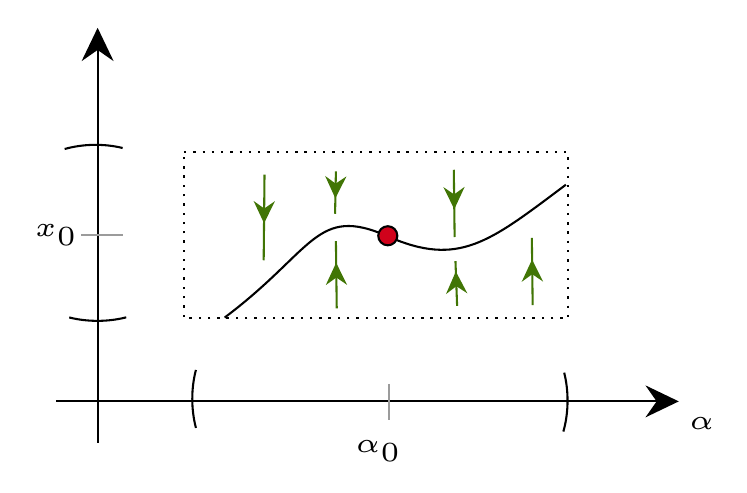
\begin{tikzpicture}[x=0.75pt,y=0.75pt,yscale=-2,xscale=2]
		%uncomment if require: \path (0,300); %set diagram left start at 0, and has height of 300
		
		%Curve Lines [id:da6170748878007859] 
		\draw    (280.6,129.8) .. controls (302.16,113.63) and (302.6,102.6) .. (319.8,110.2) .. controls (337,117.8) and (344.36,111.63) .. (362.8,97.8) ;
		%Straight Lines [id:da09861653689071792] 
		\draw    (240,150) -- (387,150) ;
		\draw [shift={(390,150)}, rotate = 180] [fill={rgb, 255:red, 0; green, 0; blue, 0 }  ][line width=0.08]  [draw opacity=0] (8.04,-3.86) -- (0,0) -- (8.04,3.86) -- (5.34,0) -- cycle    ;
		%Straight Lines [id:da21639286510164335] 
		\draw    (250,160) -- (250,63) ;
		\draw [shift={(250,60)}, rotate = 90] [fill={rgb, 255:red, 0; green, 0; blue, 0 }  ][line width=0.08]  [draw opacity=0] (8.04,-3.86) -- (0,0) -- (8.04,3.86) -- (5.34,0) -- cycle    ;
		%Shape: Arc [id:dp8981115574458696] 
		\draw  [draw opacity=0] (273.68,156.39) .. controls (273.12,154.26) and (272.8,151.89) .. (272.8,149.4) .. controls (272.8,146.92) and (273.11,144.56) .. (273.68,142.43) -- (282.8,149.4) -- cycle ; \draw   (273.68,156.39) .. controls (273.12,154.26) and (272.8,151.89) .. (272.8,149.4) .. controls (272.8,146.92) and (273.11,144.56) .. (273.68,142.43) ;  
		%Shape: Arc [id:dp06952342542904488] 
		\draw  [draw opacity=0] (362.39,143.08) .. controls (362.91,145.14) and (363.2,147.41) .. (363.2,149.8) .. controls (363.2,152.48) and (362.84,155.01) .. (362.19,157.26) -- (353.2,149.8) -- cycle ; \draw   (362.39,143.08) .. controls (362.91,145.14) and (363.2,147.41) .. (363.2,149.8) .. controls (363.2,152.48) and (362.84,155.01) .. (362.19,157.26) ;  
		%Straight Lines [id:da1271782911650352] 
		\draw [color={rgb, 255:red, 155; green, 155; blue, 155 }  ,draw opacity=1 ]   (320.2,145.8) -- (320.2,154.6) ;
		%Straight Lines [id:da39503739230709356] 
		\draw [color={rgb, 255:red, 155; green, 155; blue, 155 }  ,draw opacity=1 ]   (246,110) -- (256,110) ;
		%Shape: Arc [id:dp12989044576154574] 
		\draw  [draw opacity=0] (256.89,129.75) .. controls (254.79,130.29) and (252.46,130.59) .. (250.02,130.6) .. controls (247.58,130.6) and (245.26,130.31) .. (243.16,129.78) -- (250,120.8) -- cycle ; \draw   (256.89,129.75) .. controls (254.79,130.29) and (252.46,130.59) .. (250.02,130.6) .. controls (247.58,130.6) and (245.26,130.31) .. (243.16,129.78) ;  
		%Shape: Arc [id:dp6331916597674339] 
		\draw  [draw opacity=0] (242.06,89.2) .. controls (244.18,88.6) and (246.54,88.24) .. (249.03,88.2) .. controls (251.52,88.16) and (253.88,88.43) .. (256.02,88.96) -- (249.2,98.2) -- cycle ; \draw   (242.06,89.2) .. controls (244.18,88.6) and (246.54,88.24) .. (249.03,88.2) .. controls (251.52,88.16) and (253.88,88.43) .. (256.02,88.96) ;  
		%Shape: Rectangle [id:dp2141756481187609] 
		\draw  [dash pattern={on 0.84pt off 2.51pt}] (270.8,90) -- (363.4,90) -- (363.4,130) -- (270.8,130) -- cycle ;
		%Shape: Circle [id:dp6389280177413919] 
		\draw  [fill={rgb, 255:red, 208; green, 2; blue, 27 }  ,fill opacity=1 ] (317.6,110.1) .. controls (317.6,108.83) and (318.63,107.8) .. (319.9,107.8) .. controls (321.17,107.8) and (322.2,108.83) .. (322.2,110.1) .. controls (322.2,111.37) and (321.17,112.4) .. (319.9,112.4) .. controls (318.63,112.4) and (317.6,111.37) .. (317.6,110.1) -- cycle ;
		%Straight Lines [id:da3444362521363762] 
		\draw [color={rgb, 255:red, 65; green, 117; blue, 5 }  ,draw opacity=1 ]   (290.2,95.4) -- (290,116) ;
		\draw [shift={(290.09,107.1)}, rotate = 270.56] [fill={rgb, 255:red, 65; green, 117; blue, 5 }  ,fill opacity=1 ][line width=0.08]  [draw opacity=0] (5.36,-2.57) -- (0,0) -- (5.36,2.57) -- (3.56,0) -- cycle    ;
		%Straight Lines [id:da8243834750989563] 
		\draw [color={rgb, 255:red, 65; green, 117; blue, 5 }  ,draw opacity=1 ]   (307.4,94.6) -- (307.2,104.8) ;
		\draw [shift={(307.27,101.1)}, rotate = 271.12] [fill={rgb, 255:red, 65; green, 117; blue, 5 }  ,fill opacity=1 ][line width=0.08]  [draw opacity=0] (5.36,-2.57) -- (0,0) -- (5.36,2.57) -- (3.56,0) -- cycle    ;
		%Straight Lines [id:da11731949971207856] 
		\draw [color={rgb, 255:red, 65; green, 117; blue, 5 }  ,draw opacity=1 ]   (335.8,94.2) -- (336,110.4) ;
		\draw [shift={(335.92,103.7)}, rotate = 269.29] [fill={rgb, 255:red, 65; green, 117; blue, 5 }  ,fill opacity=1 ][line width=0.08]  [draw opacity=0] (5.36,-2.57) -- (0,0) -- (5.36,2.57) -- (3.56,0) -- cycle    ;
		%Straight Lines [id:da09921986693019402] 
		\draw [color={rgb, 255:red, 65; green, 117; blue, 5 }  ,draw opacity=1 ]   (354.6,110.6) -- (354.8,126.8) ;
		\draw [shift={(354.66,115.8)}, rotate = 89.29] [fill={rgb, 255:red, 65; green, 117; blue, 5 }  ,fill opacity=1 ][line width=0.08]  [draw opacity=0] (5.36,-2.57) -- (0,0) -- (5.36,2.57) -- (3.56,0) -- cycle    ;
		%Straight Lines [id:da6815749353841114] 
		\draw [color={rgb, 255:red, 65; green, 117; blue, 5 }  ,draw opacity=1 ]   (307.4,111.4) -- (307.6,127.6) ;
		\draw [shift={(307.46,116.6)}, rotate = 89.29] [fill={rgb, 255:red, 65; green, 117; blue, 5 }  ,fill opacity=1 ][line width=0.08]  [draw opacity=0] (5.36,-2.57) -- (0,0) -- (5.36,2.57) -- (3.56,0) -- cycle    ;
		%Straight Lines [id:da33325678105242607] 
		\draw [color={rgb, 255:red, 65; green, 117; blue, 5 }  ,draw opacity=1 ]   (336.2,116.2) -- (336.6,127) ;
		\draw [shift={(336.29,118.7)}, rotate = 87.88] [fill={rgb, 255:red, 65; green, 117; blue, 5 }  ,fill opacity=1 ][line width=0.08]  [draw opacity=0] (5.36,-2.57) -- (0,0) -- (5.36,2.57) -- (3.56,0) -- cycle    ;
		
		% Text Node
		\draw (391,152.4) node [anchor=north west][inner sep=0.75pt]  [font=\tiny,xscale=2,yscale=2]  {$\alpha $};
		% Text Node
		\draw (310.6,158) node [anchor=north west][inner sep=0.75pt]  [font=\tiny,xscale=2,yscale=2]  {$\alpha _{0}$};
		% Text Node
		\draw (233.4,106) node [anchor=north west][inner sep=0.75pt]  [font=\tiny,xscale=2,yscale=2]  {$x_{0}$};
		
		
	\end{tikzpicture}
\end{figure}